% Soft-card starting point for an ML method figure — the modern LLM/RL-report
% look (rounded cards, pastel gradient bodies, one quiet blur shadow, sans).
% The flat-journal counterpart is tikz-template.tex. Pick ONE family per
% paper and keep every figure in it. See references/method-figure/polish-style.md.
%
% Build:  xelatex -interaction=nonstopmode -halt-on-error <name>.tex
% Gate:   scripts/method-figure/qa.sh <name>.tex --venue iclr
% Render: qlmanage -t -s 2400 -o <dir> <name>.pdf   (flattens onto white)

\documentclass[tikz,border=10pt]{standalone}
\usepackage{amsmath}
\usepackage{newtxtext,newtxmath}   % math matches a Times body; labels are sans
\usepackage{fontawesome5}          % semantic glyphs only: \faSnowflake, \faFire
\usetikzlibrary{arrows.meta,bending,calc,fit,positioning,backgrounds,shadows.blur}

% ============================================================================
% PALETTE — tokens only, never inline hex below this line. One hue per ROLE.
% ink/inklight are structure; cblue is standard/frozen flow; corange is THE
% accent (the novel component); cgreen is verified/positive (small chips).
% ============================================================================
\definecolor{ink}{HTML}{334155}
\definecolor{inklight}{HTML}{94A3B8}
\definecolor{cblue}{HTML}{2563EB}
\definecolor{corange}{HTML}{D97706}
\definecolor{cgreen}{HTML}{059669}
\definecolor{cviolet}{HTML}{7C3AED}

% ============================================================================
% PARAMETERS — all spacing lives here; gaps come from this discrete set.
% ============================================================================
\newlength{\cardpad}\setlength{\cardpad}{8pt}
\def\colgap{1.1cm}   % sibling gap, horizontal
\def\rowgap{0.7cm}   % sibling gap, vertical

\begin{document}
\begin{tikzpicture}[
  font=\sffamily\small, text=ink, node distance=\colgap and \colgap,
% --- cards -----------------------------------------------------------------
  card/.style={rounded corners=5pt, draw=#1!65!black, line width=1.0pt,
      top color=#1!10, bottom color=#1!3, inner sep=\cardpad, align=center,
      blur shadow={shadow xshift=.5ex, shadow yshift=-.5ex,
        shadow blur radius=.4ex, shadow blur steps=8,
        shadow blur extra rounding, shadow opacity=30}},
  flat/.style={rounded corners=5pt, draw=#1!65!black, line width=1.0pt,
      fill=#1!8, inner sep=\cardpad, align=center},
% --- header pill / chips -----------------------------------------------------
  hdrpill/.style={fill=#1!75!black, text=white, rounded corners=6pt,
      font=\sffamily\bfseries\footnotesize, inner xsep=8pt, inner ysep=3.5pt},
  chip/.style={rounded corners=7pt, draw=#1!65!black, line width=0.7pt,
      fill=#1!10, text=#1!55!black, font=\sffamily\scriptsize,
      inner xsep=6pt, inner ysep=2.5pt},
  note/.style={font=\sffamily\scriptsize, text=inklight, align=center},
% --- arrows: three weights, geometric round tips ------------------------------
  flow/.style={-{Stealth[length=2.2mm,width=1.7mm,round]}, line width=1.1pt,
      draw=ink, line cap=round, shorten >=1.5pt, shorten <=1pt},
  thinflow/.style={flow, line width=0.6pt, draw=inklight,
      -{Stealth[length=1.6mm,width=1.2mm,round]}},
  emphflow/.style={flow, line width=1.7pt, draw=#1},
  emphflow/.default=corange,
]
% NOTE: no blank lines inside a tikzpicture. Rounded orthogonal elbows:
% \draw[flow, rounded corners=6pt] (a.east) -| (b.north);
% ---- content -----------------------------------------------------------------
\node[card={cblue}] (teacher) {\faSnowflake[regular]\; frozen teacher\\[2pt]
  $q^{\mathrm{GT}}(v\mid h_t)$};
\node[hdrpill={cblue}, above=0.5cm of teacher] (teacher-title) {privileged branch};
\draw[flow] (teacher.east) -- +(1.2,0);
% ---- flatten the page onto white (keeps sips/QA renders honest) --------------
\begin{scope}[on background layer,overlay]
  \fill[white] ($(current bounding box.south west)+(-12pt,-12pt)$)
    rectangle ($(current bounding box.north east)+(12pt,12pt)$);
\end{scope}
\end{tikzpicture}
\end{document}
